
% to choose your degree
% please un-comment just one of the following

\documentclass[bsc,frontabs,twoside,singlespacing,parskip,deptreport]{infthesis}     % for BSc, BEng etc.
% \documentclass[minf,frontabs,twoside,singlespacing,parskip,deptreport]{infthesis}  % for MInf

\usepackage{bm}
\usepackage[thinc]{esdiff}
\usepackage{todonotes}
\usepackage{mathrsfs}
\usepackage{amsmath}
\usepackage{amssymb}
\usepackage{booktabs}
\usepackage{subcaption}
\usepackage{placeins}

\let\Oldsection\section
\renewcommand{\section}{\FloatBarrier\Oldsection}

\let\Oldsubsection\subsection
\renewcommand{\subsection}{\FloatBarrier\Oldsubsection}

\let\Oldsubsubsection\subsubsection
\renewcommand{\subsubsection}{\FloatBarrier\Oldsubsubsection}

%\reversemarginpar
\begin{document}

\title{An Interpretable Deep Learning Approach to Pharmacodynamic Mechanism of Action Prediction using Transcriptomic Data}

\author{Ragnor Comerford}

% to choose your course
% please un-comment just one of the following
\course{Artificial Intelligence and Computer Science}
%\course{Artificial Intelligence and Software Engineering}
%\course{Artificial Intelligence and Mathematics}
%\course{Artificial Intelligence and Psychology }   
%\course{Artificial Intelligence with Psychology }   
%\course{Linguistics and Artificial Intelligence}    
%\course{Computer Science}
%\course{Software Engineering}
%\course{Computer Science and Electronics}    
%\course{Electronics and Software Engineering}    
%\course{Computer Science and Management Science}    
%\course{Computer Science and Mathematics}
%\course{Computer Science and Physics}  
%\course{Computer Science and Statistics}    

% to choose your report type
% please un-comment just one of the following
\project{Undergraduate Dissertation} % CS&E, E&SE, AI&L
%\project{Undergraduate Thesis} % AI%Psy
%\project{4th Year Project Report}

\date{\today}

\abstract{
Mechanism of action prediction is the task of inferring the biological activity of compounds in drug discovery.\\
This works explores the applicability of deep neural networks for this inference task. Existing approaches applying deep learning to drug discovery tasks are reviewed and discussed. A system for optimizing the neural networks using Bayesian Optimization is designed and evaluated with promising results.
Lastly, a method is proposed that employs integrated gradient allowing for biological interpretations of the model predictions.
}

\maketitle

\section*{Acknowledgements}
I would like to express my sincere gratitude to my supervisor, Michael Herrmann, for his valuable guidance and insightful feedback. I would also like to thank my family and friends for their constant support and love
throughout my academic years.

\tableofcontents

%\pagenumbering{arabic}


\chapter{Introduction}

\section{Motivation}
Drug discovery has traditionally been an expensive and inefficient process with a very serendipitous approach to the identification of novel drug compounds.
Despite the huge scientific and technological advances such as high-throughput screening (HTS), parallel synthesis and combinatorial chemistry in the past decade, the biopharmaceutical industry has not seen much increase in efficiency. This development, coined \textit{Eroom's Law}, states that drug discovery has become slower and more expensive with a steadily decrease in efficiency since the 1980s \cite{scannell_diagnosing_2012}. But it is as much an issue of science as it is a social and political one. The cost of each new molecular entity (NME) has climbed to approximately US\$1.8 billion \cite{paul_how_2010}. as "the number of new drugs approved per billion US dollars spent on R\&D has halved roughly every 9 years since 1950, falling around 80-fold in inflation-adjusted terms"\cite{scannell_diagnosing_2012}.
The astronomical costs of drug development are reflected in the inequality of access to health care and disproportionately affects developing countries where a big proportion of the population is deprived of life-saving treatment. \\
However, recent advances in machine learning (ML) coupled with a significant increase in computing power and data are inducing a renaissance in drug development.
Deep learning (DL) \cite{lecun_deep_2015} with its ability to model complex non-linear relationships has successfully taken advantage of the exponential growth in the availability of data and computer hardware. The algorithmic optimization of DL algorithms for graphical processing units (GPUs) has significantly reduced the time to train DL models by leveraging the power of GPUs to significantly speed up parallel processing and matrix operations.
The explosive growth of available biomedical and compound activity databases \cite{papadatos_activity_2015}\cite{kim_pubchem_2016}\cite{gaulton_chembl_2012}, partly owed to the emergence of new experimental techniques such as HTS or parallel synthesis \cite{grada_next-generation_2013}, allows DL to perform automatic feature detection and complex representation learning from massive amounts of unlabelled or labelled biomedical data.\\
One such instance of large-scale biomedical data collection enabled by new experimental techniques is the \textit{Connectivity Map} (CMap) \cite{lamb_connectivity_2006} which plays a central role in our work. The CMap is a project within the Broad Institute of MIT and Harvard, the Laboratory for Innovation Science at Harvard (LISH), and the  NIH  Common  Funds  Library  of  Integrated  Network-Based  Cellular  Signatures (LINCS) that uses gene expression signatures to discover functional connections among diseases, genetic perturbation, and drug action \cite{musa_review_2017}. They developed the L1000 assay to facilitate rapid, flexible and high-throughput gene expression profiling at lower costs \cite{subramanian_next_2017} and built a comprehensive, large-scale drug perturbation database containing gene expression signatures of a wide range of cultivated cell lines treated with thousands of chemical compounds. In this work, we leverage the recent availability of such data as well as deep learning techniques to understand the relationship between drugs, genes and pathways and build an accurate model predicting the function of unknown compounds.


\section{Contributions}
\begin{itemize}
\item Literature review on existing approaches to drug action prediction 
\item Correlation and Principal Component Analysis
\item Design and implementation of neural networks for mechanism of action prediction
\item Implementation of Bayesian Optimization
\item Biological interpretation of the learned model using the feature attribution method \textit{Integrated Gradients}

\end{itemize}

\chapter{Background}
In this chapter, we introduce the reader to the biological concepts and mechanisms that are relevant to the understanding of deep learning applications to drug discovery. This is followed by a brief introduction to deep learning algorithms. \\
For more comprehensive introductions, we refer the interested reader to Goodfellow \textit{et al.} (2016) \cite{goodfellow_deep_2016} and Alberts \textit{et al.} (2013) \cite{alberts_essential_2013}/
\section{Molecular biology}
\subsection{Gene expression}
\textit{Gene expression} forms the fundamental part of the central dogma of microbiology \cite{crick_protein_1958} and refers to the process by which the genetic information stored in the DNA is used in the synthesis of a gene product such as RNA or protein. Gene expression can be regulated by a wide range of biological mechanisms in the cell. Activation or inactivation of signaling pathways in regular physiological processes or in response to stimuli affects gene expression via transcription factors and their regulatory genes \cite{itadani_can_2008}. This cascade of signal transduction generates characteristic patterns of gene expression, commonly referred to as \textit{gene expression signatures}.
Changes in gene expression as a consequence of disease or pharmacologic perturbation (termed \textit{differential gene expression signatures}) bears significant potential in improving our understanding of disease treatment and the identification of drug targets.
\subsection{Cell viability}
\textit{Cell viability} is a measure of metabolically active (living) cells within a population. Cell viability assays can be used to measure cell survival or cell health following treatment with compounds such as drugs or exposure to experimental conditions. Compounds that are toxic to cells are referred to as \textit{cytotoxic}.
\subsection{Mechanism of Action}
The \textit{mechanism of action} (MoA) of a compound refers to the set of target and effector proteins that are associated with a particular biological activity in a specific cellular context. Its correct identification for novel compounds represents a major challenge in drug development as most candidate compounds fail in the pharmacological pipeline due to toxicity associated with off-target affects and lack of efficacy \cite{wehling_assessing_2009}. Additionally, knowledge about the MoA allows drugs to be combined in a way that reduces the likelihood of drug resistance by inhibiting multiple targets simutaneously \cite{bozic_evolutionary_2013}. It can also help identify which patients are most likely to respond to treatment based on the presence of the target molecules in the patient \cite{noauthor_mechanism_2010}. Finally, it allows existing drugs to be re-purposed for the treatment of other diseases with shared MoA \cite{meninger_webcast_nodate}.


\section{Deep learning}
\textit{Deep learning} can generally be described as a class of machine learning algorithms that uses \textit{artificial neural networks} (ANNs) with multiple layers between the input and output layers for learning data representations. ANNs are loosely inspired by the biological brain where inter-connected neurons transmit signals to each other.
The universal approximation theorem represents an important discovery in the theory of deep learning. It states that, for any continuous function \(f\) on a compact space \(K\), there exists a single-hidden-layer feedforward neural network which uniformly approximates \(f\) within an arbitrary error \(\epsilon>0\) on \(K\) \cite{hornik_multilayer_1989}. However, in practice, it is often favourable to use multiple hidden layers as it greatly reduces the size of the network and the need for data to learn representations that generalise well.

\subsection{Feedforward neural network}
A \textit{feedforward neural network} consists of an input layer and output layer that passes information in a forward fashion through a series of latent layers with the ultimate goal of approximating a function with a composition of intermediate computations. More formally, a feedfoward neural network, also called \textit{multilayer perceptron}, approximates some function \(f'\) by learning the values of parameters \(\mathbf{\theta}\) such that \(f(\mathbf{x} ; \mathbf{\theta}) \approx f'\).
Each layer \(l\) in the feedforward neural network consists of a linear combination of the previous layer \(l-1\), followed by a non-linear transformation \(g^{(l)}\) such that 
% \[\bm{h^{(l)}} = g^{(l)}(W^{(l)}\bm{h^{(l-1)}} + \bm{b^{(l)})},\]

\[a_{j}^{(l)}=\sum_{i} w_{j i}^{(l)} z_{i}^{(l-1)}+b_{j}^{(l)}\]

\[z_{j}^{(l)}=g^{(l)}\left(a_{j}^{(l)}\right)\]

where \(w\) represents the weights and \(b^{(l)}\) the bias allowing a shift in the activation. The logistic sigmoid is a very commonly used activation function: \[g^{(l)}(a) = \sigma(a) = \frac{1}{1+e^{-a}}\]
Other common functions include the Rectified Linear Unit (ReLu), \(g^{(l)}(a)= \max(0, a)\), the hyperbolic tangent, \(g^{(l)}(a)={\frac {e^{a}-e^{-a}}{e^{a}+e^{-a}}}\), or the radial basis function, \(g^{(l)}(a)=\varphi (\left\|a -c \right\|)\), where \(\varphi\) is a positive definite function with shape parameter \(\varepsilon\) such as the Gaussian \(\varphi(r)=e^{-(\varepsilon r)^{2}}\).
\subsection{Training}
For a given dataset \(X\), the typical training procedure of a feedforward neural network parameterized by \(\theta\) is gradient-based and consists of a series of steps: \\
\begin{enumerate}
    \item{ \bf{Defining a differentiable loss function}} \vspace{0.2cm} \\
    The choice of the loss function \(E_{\theta}(\mathbf{X})\) is an important aspect of network training and is typically selected such that \(E_{\theta}(\mathbf{X})\) is small when \(f_{\theta}(\mathbf{X}) \approx f'\). In a probabilistic interpretation, the appropriate loss function for a given problem can be derived from the principle of maximum likelihood estimation. For regression problems, maximising the likelihood by assuming a Gaussian noise distribution \(\epsilon\sim N(0,1)\) with 0 mean and unit variance on the output yields the so-called \textit{mean-squared (MSE) loss}. For \(N\) samples with input feature \(\mathbf{x}_{i}\) true label \(\mathbf{y}_{i}\) we define it as
    
\begin{equation}
MSE=\frac{1}{N} \sum_{i=1}^{N}\left\|\mathbf{y}_{i}-f_{\theta}(\mathbf{x}_{i}) \right\|^{2}
\end{equation}

In the context of binary classification, we interpret the squashed output scalar \({y}_{i}\) of the network as a probability and assume that the data are independent and identically distributed, yielding the likelihood
\begin{equation}
L(X)=\prod_{i=1}^{N}\left[f_{\theta}\left(\mathbf{x}_{i}\right)\right]^{\left({y}_{i}\right)}\left[1-f_{\theta}\left(\mathbf{x}_{i}\right)\right]^{\left(1-{y}_{i}\right)}
\end{equation}
    
For mathematical convenience, we take the logarithm of the expression and obtain our classification loss function, the \textit{cross-entropy loss}.

\begin{equation}
CE = -\sum_{i=1}^{N} y_{i} \log \left(f_{\theta}\left(\mathbf{x}_{i}\right)\right)+\left(1-y_{i}\right) \log \left(1-f_{\theta}\left(\mathbf{x}_{i}\right)\right)
\end{equation}

We can generalise to multi-class classification, which we are using in chapter 5, by one-hot encoding our labels \(\mathbf{y}_{i}\) for \(K\) classes:

\begin{equation}
   CE = -\sum_{i=1}^{N} \sum_{j=1}^{K} y_{i j} \log \left(f_{\theta}\left(x_{i}\right)_{j}\right)+\left(1-y_{i j}\right) \log \left(1-f_{\theta}\left(x_{i}\right)_{j}\right)
\end{equation}

    
    \item{ \bf{Computing the loss gradients} } \\
    \textit{Backpropagation} (also known as \textit{back-propagation of error}, or \textit{back-prop}) \cite{rumelhart_learning_1986} is by far the most popular and widely used algorithm for computing the gradients of the loss function of neural networks. Backpropagation is an instance of automatic reverse-mode differentiation and gained its popularity from the fact that it can accumulate all of the partial derivatives of any function with respect to all of its input in a very efficient manner. 

By repeated use of the chain rule, we can, for the squared error, compute the error signals \(\delta\) starting from the output units.
\begin{equation}
    \delta_{k}^{(L)}=2\left(z_{k}^{(L)}-y_{k}\right) \cdot g^{(L)\prime}\left(a_{k}^{(L)}\right)
\end{equation}

The hidden unit error signals are then given by
\begin{equation}
    \delta_{j}^{(l)}=g^{(l)\prime}\left(a_{j}^{(l)}\right) \sum_{k} w_{k j}^{(l+1)} \delta_{k}^{(l+1)}.
\end{equation}


Finally, the derivatives with respect to the model parameters are given by
\begin{equation}
    \frac{\partial E}{\partial w_{k j}^{(l)}}=\delta_{k}^{(l)} z_{j}^{l-1} \quad\quad \frac{\partial E}{\partial b_{k}^{(l)}}=\delta_{k}^{(l)}
\end{equation}

    
    
    
    
%     Given the computation graph \[\begin{array}{cccl}
%   \cdots \rightarrow & \!\!A\!\! &          & \\
% &           & \searrow & \\
% &           &          & \!\!C \rightarrow \cdots \rightarrow z\\
% &           & \nearrow & \\
% \cdots\rightarrow & \!\!B\!\! &          & \\
% \end{array}\]
% where the matrices \(A\) and \(B\) are multiplied to form the matrix \(C\) which is then transformed to the scalar \(z\), we can derive the general equation for backpropagating the matrix derivative \(\bar{A}_{i j}\) using the chain rule:
% \[\bar{A}_{i j}=\frac{\partial z}{\partial A_{i j}}=\sum_{k, l} \frac{\partial z}{\partial C_{k l}} \frac{\partial C_{k l}}{\partial A_{i j}}=\sum_{k, l} \bar{C}_{k l} \frac{\partial C_{k l}}{\partial A_{i j}}\]

% \[\frac{\partial E}{\partial W_{i j}}=\frac{\partial E}{\partial y_{i}} \frac{\partial y_{i}}{\partial g} \frac{\partial g}{\partial W_{i j}}\]

    % \todo[inline]{Briefly explain backpropagation}
    %  \(\diffp{E(X,\theta)}{\theta}\)
     
     
    \item{ \bf{Optimization} } \\ 
    The final traning step consists of an optimization procedure to perform learning using the gradient, i.e., minimize the error function. The most popular optimization algorithm used is \textit{Stochastic Gradient Descent} (SGD). It performs the following update of parameter \(\theta\) for each training pair \((\mathbf{x}_i,\mathbf{y}_i)\):
    \begin{equation}
   \theta=\theta-\eta \cdot \nabla_{\theta} E\left(\theta ; \mathbf{x}_i ; \mathbf{y}_i\right),\end{equation}
    where \(\eta\) denotes the learning rate that determines the size of the steps we take to reach a (local) minimum \cite{ruder_overview_2017}. In neural networks, the parameters to be updated are the weights and biases.\\ There exists a wide range of other algorithms that try to improve the speed of convergence, the vulnerability to local optima and other properties of the learning procedure. One such popular algorithm is the adaptive learning rate method \textit{Adam} \cite{ruder_overview_2017}. It uses estimations of first and second moments of the gradient to adapt the learning rate for each parameter \cite{ruder_overview_2017}.
    
\end{enumerate}

  



\subsection{Regularization by Dropout}
Deep neural networks can have a very large number of parameters and are hereby vulnerable to overfitting. Neural units commonly suffer from co-adaptation as they influence each other through the backpropagated derivative that is used to optimize the network \cite{srivastava_dropout_2014}. The co-adaptations do not generalise well to unseen data, causing the network to overfit. A useful technique for addressing this issue is dropout which randomly drops units and their connections during training \cite{srivastava_dropout_2014}. This makes the presence of other hidden units unreliable and  leads to sparse representations in the network \cite{srivastava_dropout_2014}. The appropriate probability of dropout depends on the task and is commonly optimized in hyperparamereter tuning.



\section{Related Work}
The three most prevalent applications of deep learning to drug discovery are \textit{de novo} drug design, drug-target interaction prediction (DTI), and compound property and activity prediction. \\ 
 \textit{De novo} drug design takes a generative approach by using neural networks to design novel molecules with certain desired properties. Gomez-Bombarelli \textit{et al.} proposed a method \cite{gomez-bombarelli_automatic_2018} that uses variational autoencoders (VAE) to learn continuous latent representations of string-encoded chemical structures coined SMILES (Simplified molecular-input line-entry system). After identifying optimal solutions in the latent space, the continuous vector representations are transformed back into string-encoded chemical structures, hereby generating new potential compounds.
 However, this method has the disadvantage of potentially yielding invalid molecules. Kusner \textit{et. al.} addressed this issue by introducing \textit{grammar variational autoencoders} (GVAE) \cite{kusner_grammar_2017} which
encode and decode directly to and from parse trees from a \textit{context-free grammar} (CFG). Jaques \textit{et al.} built on the success of recurrent neural networks (RNNs) in the field of natural language processing and \textit{Reinforcement Learning} (RL). They generated SMILES strings using RNNs and applied the RL method \textit{Deep Q-Learning} to incite desired, domain-specific properties \cite{jaques_sequence_2017}. \\
Drug-target interaction prediction (DTI) is another prominent approach in drug discovery and is concerned with the recognition of interactions between chemical compounds and the protein targets in the human body. Modulation of protein structure and function induced by interactions with compounds can have dramatic effects on the body as proteins are involved in a plethora of biological processes and pathways. Therefore, accurate interaction predictions can yield important discoveries on suitable drug candidates.
Feng \textit{et al.} employed deep learning methods to predict DTI. They combined Molecular Graph Convolution (MGC) for compound featurization with protein descriptors to predict real-valued interaction strength between compounds and proteins \cite{feng_padme_2019}.
Ragoza \textit{et al.}  proposed a method for protein-ligand scoring that applies a \textit{Convolutional Neural Network} (CNN) to three-dimensional (3D) representations of protein-ligand interactions as input. The scoring function automatically learns the key features of the protein-ligand interactions that correlate with binding \cite{ragoza_proteinligand_2017}. \\
The third approach, which we are primarily concerned with in this work, is the prediction of compound activities and properties. ANNs have shown significant success in recent work: Inter alia, Dahl \textit{et al.} show that deep neural networks (DNN) outperformed standard Random Forests (RF) in predicting the biological activity of compounds from numerical chemical descriptors on the Merck Kaggle challenge data set \cite{ma_deep_2015}. In particular, they established that
\begin{itemize}
    \item DNNs can learn from a large number of descriptors without feature selection,
    \item the overfitting problem can be mitigated by dropout,
    \item the optimization of hyperparameters controlling the learning procedure and neural architecture can maximise the performance of DNNs\cite{chen_rise_2018}.
\end{itemize}
However, current approaches are not sufficient to establish the causality of drug-activity pairs. Truly understanding cellular function and pathways requires perturbating biological systems and monitoring the downstream consequences. Furthermore, most work lack the interpretability of the developed models required for medical decision making. In this work, we aim to address these challenges by performing interpretable deep learning on drug perturbational data provided by the Connectivity Map.

\chapter{Experimental Setup}\label{methodology}

\section{Data}
Our data is provided by the \textit{Connectivity Map}, a project within the Broad Institute of MIT and Harvard, the Laboratory for Innovation Science at Harvard (LISH), and the NIH Common Funds Library of Integrated Network-Based Cellular Signatures (LINCS) and was generated by treating a sample of human cells with different drugs and then analyzing the cellular responses. \\ Cellular responses were measured in terms of expression levels of 772 landmark genes using the high-throughput gene expression assay L10000 and the viability values of 100 individual cell lines using the PRISM assay.\\
Formally, the data can be denoted as \(\mathscr{D}=\{\mathbf{x}^{(i)},\mathbf{y}^{(i)}\}_{i=1}^{N}\) where each tuple represents a drug perturbation, i.e., a single treatment of a sample of cells by a specific drug.
\\ Each feature vector \(\mathbf{x}^{(i)}=[\mathbf{e}^{(i)},\mathbf{v}^{(i)}, c^{(i)},d^{(i)},t^{(i)}]^{L}\) consists of 
\begin{itemize}
    \item the expression levels \(\bf{e} \in \mathbb{R}^\mathnormal{E}\) of the \(E=772\) landmark genes
    \item the cell viability values \(\bf{v} \in \mathbb{R}^\mathnormal{V}\) of the \(V=100\) different cell lineages
    \item the variable \(c \in \{0,1\}\) indicating control perturbations (\(c=1\)) or drug treatments (\(c=0\))
    \item the dose \(d \in \{0,1,2\}\)
    \item the time (in hours) \(t \in \{24,48,72\}\) of measurement after adding the compound
    
\end{itemize}

\(\mathbf{y}^{(i)}=[y_{1}^{(i)},y_{2}^{(i)},\ldots, y_{k}^{(i)}]^{K}\) denotes a one-hot encoded vector of the mechanisms of action \(y_{i}\) associated with the drug. A single perturbation can have multiple mechanisms of actions assigned


The gene expression and cell viability data was first pre-processed using quantile normalization in order to standardize the feature values across plates. Then, a robust \(z\)-score was computed for each gene based on control perturbation (drugs without any mechanism of action) values, i.e., normalized for difference from the controls (\textit{differential expression}).

\section{Problem and Task Definitions}
\begin{enumerate}
    \item Perform correlation analysis and dimensionality reduction on the feature space in order to guide our further work.
    \item Train and optimize a model to infer mechanism of action from perturbational data. More formally, we want to learn a functional mapping 
    \begin{equation} \label{funcmap}
    f: \mathbb{R}^{L} \rightarrow \mathbb{R}^{K} \text { that fits }\left\{\mathbf{x}_{i}, \mathbf{y}_{i}\right\}_{i=1}^{N}\end{equation}
    \item Interpret the model predictions with respect to the biological domain.
\end{enumerate}



\chapter{Exploratory Data Analysis}

% \begin{figure}[h!]
% \caption{Distributions of controls, dose and time.}
% 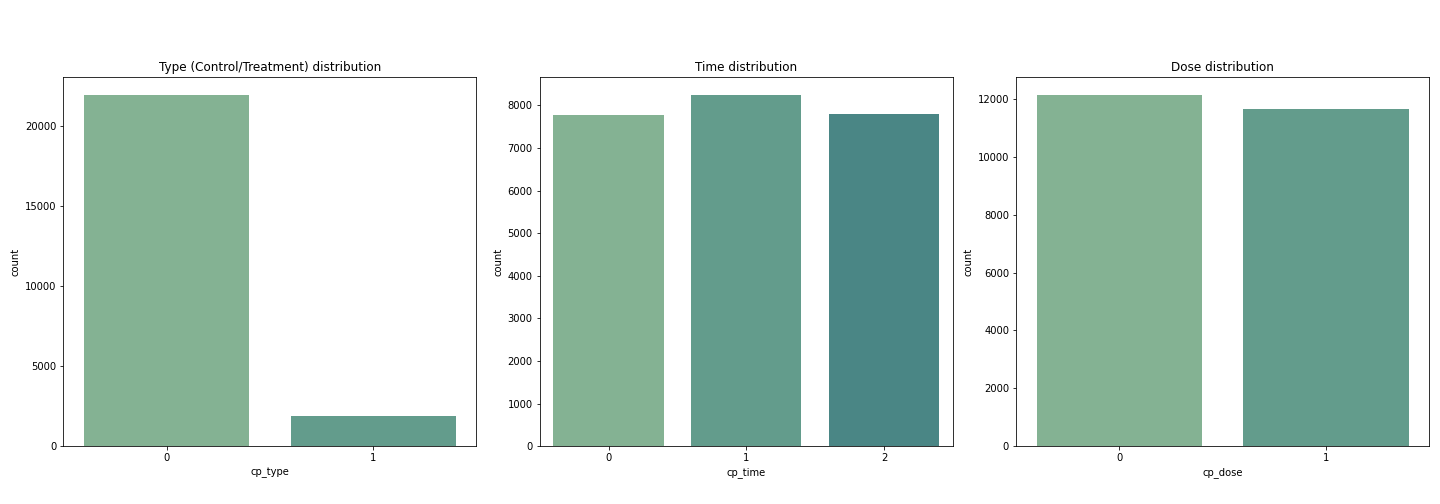
\includegraphics[height=6cm]{images/dist_plot.png}\label{cat_dist}
% \end{figure}
% \begin{figure}[h!]
% \caption{Distributions of label counts}
% 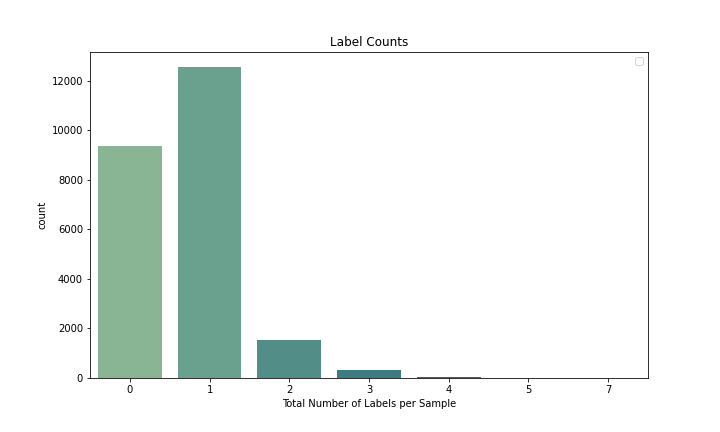
\includegraphics[height=6cm]{images/label_counts.png}\label{label_counts}
% \end{figure}

\section{Correlation Analysis}
We computed the intraclass Pearson correlation for all cell features \(\mathbf{v}\) and gene features \(\mathbf{e}\) respectively, and extracted the 35 features with highest correlation to perform agglomerative clustering with Euclidean distance. Figure \ref{corr_maps} shows heatmaps of the correlation matrices with the respective clusters.  \\
It can be clearly seen that the cell features (Figure \ref{cell_map}) do not exhibit clear clusters whereas the gene features (Figure \ref{corr_map}) contain two distinct clusters. 
\begin{figure}[h!]
\centering
\begin{subfigure}{.5\textwidth}
  \centering
  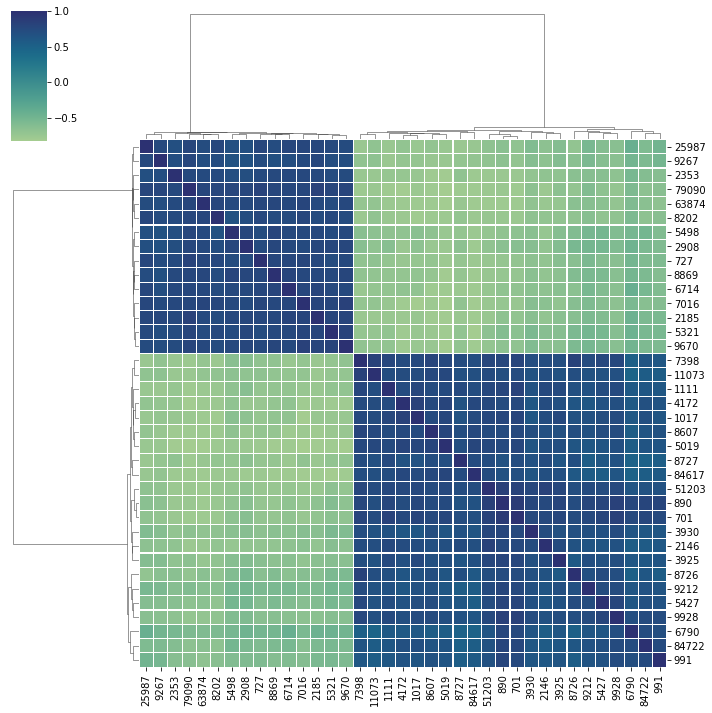
\includegraphics[width=.9\linewidth]{images/gene_corr.png}
  \caption{Genes}
  \label{gene_map}
\end{subfigure}%
\begin{subfigure}{.5\textwidth}
  \centering
  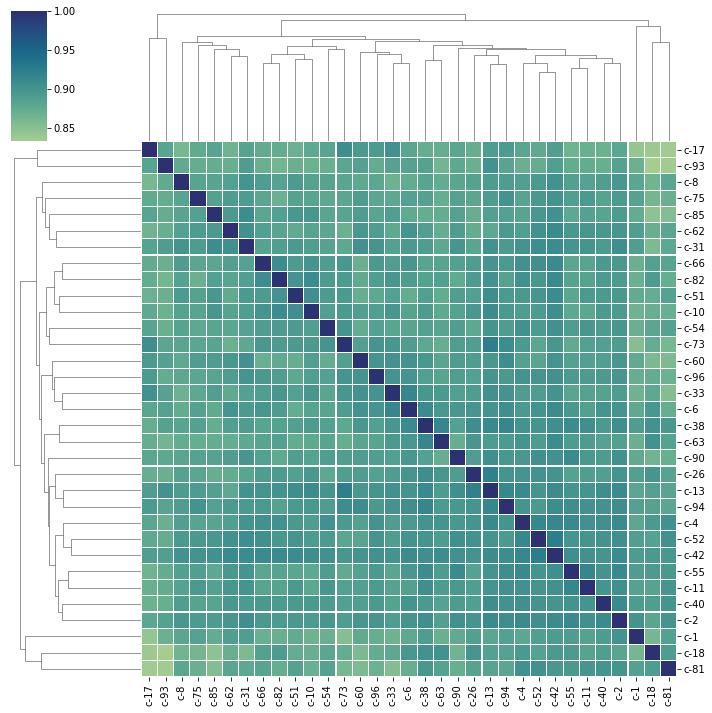
\includegraphics[width=.9\linewidth]{images/cell_corr.png}
  \caption{Cells}
  \label{cell_map}
\end{subfigure}
\caption{\textbf{Correlation maps with clusterings.} The labels correspond to unique database identifiers.}
\label{corr_maps}
\end{figure}
In order two obtain a biological interpretation of the clusters, we performed \textit{Reactome} pathway enrichment analysis on the two cluster separately. \cite{fabregat_reactome_2017}. Reactome is a peer-reviewed pathway database and the enrichment provides us with the statistically over-represented pathways in which the genes in the respective clusters are involved, hereby enabling a biological interpretation of the clusters.\\
Table \ref{c1_enrichment} and \ref{c2_enrichment} show the pathways with their associated p-values of the statistical over-representation test and clearly indicate that the clusters represent clear and distinct biological functions. The first cluster revolves around the transcription and expression of genes whereas the second cluster revolves around the cell cycle.\\
The cell cycle mainly controls cellular growth, development, and differentiation and is hereby a very common target in anticancer drug discovery \cite{bai_cell_2017}. Similarly, manipulation of protein-protein interaction is a promising avenue in pharmacology and can be induced by modulation of transcription activity \cite{fontaine_pharmacological_2015}.

\begin{table}[h!]

\centering
\begin{tabular}{ll} 
\toprule
Pathway name  & p-Value \\
\midrule
Nuclear Receptor transcription pathway & $7.14e-14$ \\
Generic Transcription Pathway &  $1.76e-5$ \\
RNA Polymerase II  Transcription &  $4.17e-5$ \\
Gene expression (Transcription) &  $1.01e-4$ \\
\bottomrule
\end{tabular}
\caption{Enrichment of cluster 1}\label{c1_enrichment}


\end{table}

\begin{table}[h!]
\centering
\begin{tabular}{ll} 
\toprule
Pathway name & p-Value \\

\midrule
Cell Cycle & $1.29e-10$ \\
Regulation of mitotic cell cycle & $2.48e-8$ \\
APC/C-mediated degradation of  cell cycle proteins & $2.48e-8$ \\
Regulation of TP53 Activity through Phosphorylation & $3.22e-8$ \\
Cell Cycle, Mitotic & $5.55e-8$ \\

\bottomrule
\end{tabular}
\caption{Enrichment of cluster 2}\label{c2_enrichment}
\end{table}


\subsection{Gene-Cells}
In order to investigate the relationship between gene expression and cell viability as a consequence of drug perturbation we computed for each sample the mean of the gene expression vector \(\mathbf{e}\) and cell viability vector \(\mathbf{v}\) respectively. We then examine pairs of scatter plots with signatures from cytotoxic perturbations (i.e., low cell viability mean) and non-cytotoxic perturbations (i.e high cell viability mean) respectively. We made consistent observations, as exemplified in Figure \ref{low_mean} and \ref{high_mean}: An increase in cytotoxicity of a compound  seems to be associated with an increase in the variability of expression levels across genes.
\begin{figure}[h!]
\centering
\begin{subfigure}{1\textwidth}
 \centering
\caption{low cell viability mean}
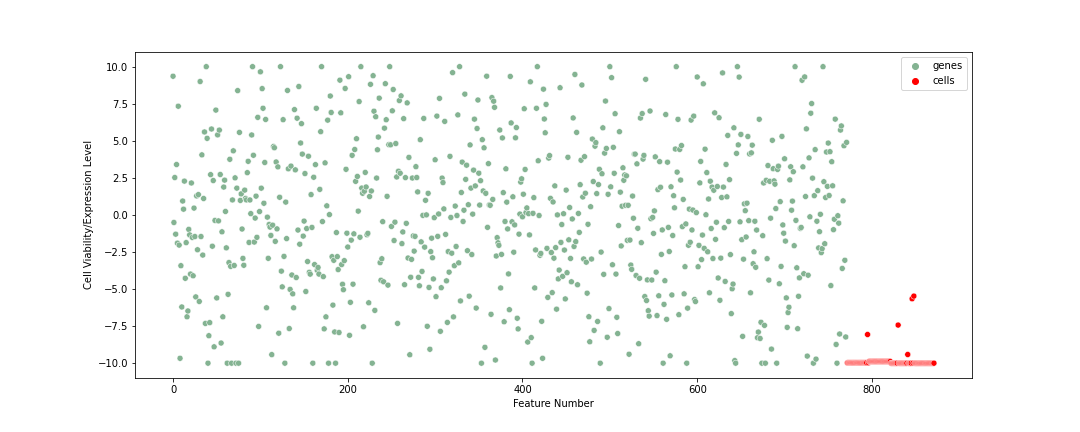
\includegraphics[height=5cm]{images/low_cell_mean.png}\label{low_mean}
\end{subfigure}
\begin{subfigure}{1\textwidth}
\centering
\caption{high cell viability mean.}
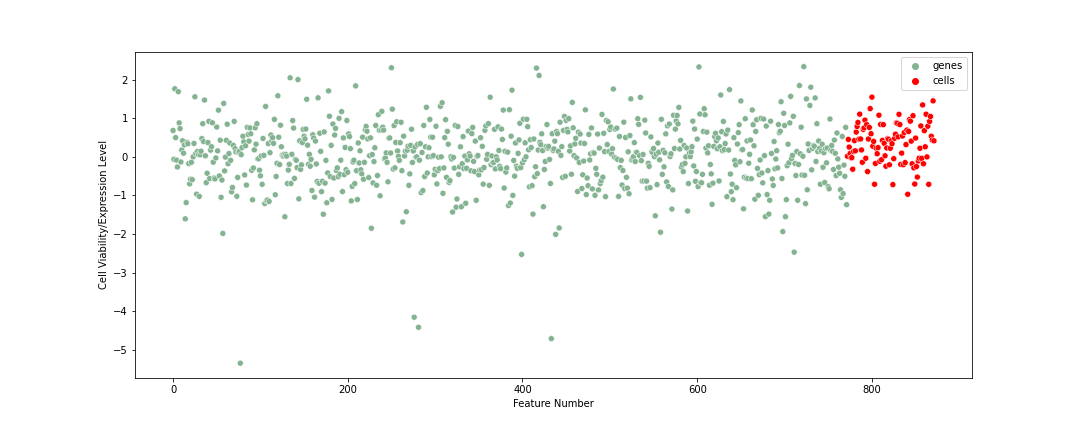
\includegraphics[height=5cm]{images/high_cell_mean.png}\label{high_mean}
\end{subfigure}
\caption{\textbf{Scatter plot of samples.} The x-axis shows the individual features of the sample and the y-axis the associated feature values.}
\end{figure}
\clearpage
In order to statistically solidify this observation, we  measured the Pearson correlation between the cell viability mean and the standard deviation of the gene expression means and could identify a statistically relevant correlation of -0.8836 (\(p\leq1e-6\)). This suggest that cell death is strongly associated with changes in gene expression.
We further found that the cell viability does not correlate with the gene expression mean (\(p\leq1e-6\)) but, instead, correlates highly with the absolute gene expression mean (\(p\leq1e-6\)) indicating that perturbation induced cell death is not associated with up- or down- regulation of genes specifically but with regulation in general. 

\begin{figure}[h!]
\centering
\caption{Heatmap of Pearson Correlations of feature statistics.}
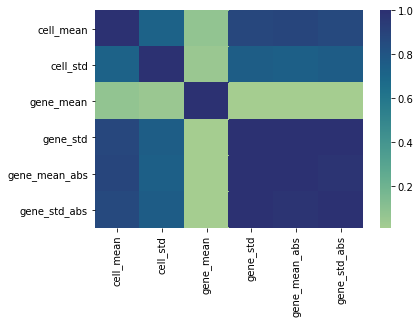
\includegraphics[height=7cm]{images/gene_cell_corr.png}\label{corr_map}
\end{figure}
\begin{table}[h!]
\centering
\begin{tabular}{lrrrr}
\toprule
{} &  cell mean &  cell std &  gene mean &  gene std \\
\midrule
cell mean &   1.000000 & -0.729786 &   0.079834 & -0.883603 \\
cell std  &  -0.729786 &  1.000000 &  -0.052747 &  0.755585 \\
gene mean &   0.079834 & -0.052747 &   1.000000 &  0.010411 \\
gene std  &  -0.883603 &  0.755585 &   0.010411 &  1.000000 \\
\bottomrule
\end{tabular}
\caption{Correlations between gene and cell statistics}\label{cell_gene_corr_table}
\end{table}

\subsection{Discussion}
The directionality of the causal relationship between regulation and cell death cannot be established from the correlations alone, but studies suggest that transcription factors may be involved in regulating cell death and profileration and that, hence, the expression signatures may be predictive of the cell viability signatures. Szalai \textit{et al.} studied similar petrurbation-based gene expression and cell viability signatures and statistically identified pathway and transcription factor activities associated with the gene–cell viability correlations. Some of the most activated (e.g. TP53, FOXO3) and inactivated (e.g. E2F1, FOXM1 and MYC) transcription factors were found to exhibit causal roles as regulators in cell death and proliferation \cite{szalai_signatures_2019}.

These findings bear significance for the inference of mechanism of action from perturbation signatures because the expression of several genes acts as a confounding factor.


\section{Dimensionality Reduction}
Principal Component Analysis (PCA) is a dimensionality reduction technique that constructs a lower-dimensional linear subspace by using an orthogonal transformation to convert a set of random variables to a set of values of linearly independent variables, called principal components (PC). The variance that is retained under the projection is hereby maximal.\\
\subsection{Results}
We performed PCA on our dataset, extracted the first two principal components and plotted the projections as shows in Figure \ref{pca map}. We can observe that the first principal component clearly separates the samples that are inhibitors of the protein complex \textit{nuclear factor kappa-light-chain-enhancer of activated B cells} (NF-kB) and hereby captures 41.8\% (Figure \ref{cum_cvar}) of the variance. The second principal component captures the separation \textit{cyclin-dependent kinase inhibitors} which are used to treat cancers by preventing overproliferation of cancer cells, hereby explaining 3.88\% of the variance.\\
We further note in plot \ref{cum_cvar} that even the first 100 principal components only manage to capture under 80\% of the cumulative variance in the data.
\begin{figure}[h!]
\centering
\begin{subfigure}{.9\textwidth}
 
  \centering
  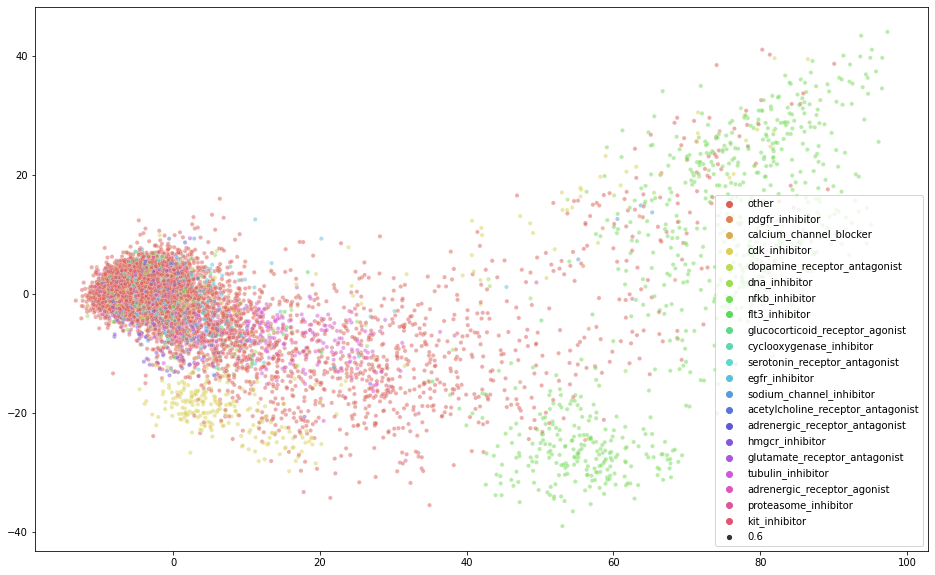
\includegraphics[width=1\linewidth]{images/pca.png}
  \caption{\textbf{Data projection onto the first two principal components}. PC 1 appears to capture the variance explaining the separation of nfkb inhibitors.}
  \label{pca map}
\end{subfigure}
\begin{subfigure}{.9\textwidth}
  \centering
  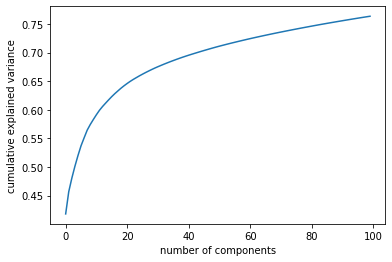
\includegraphics[width=.6\linewidth]{images/cum_variance.png}
  \caption{Cumulative variance explained by the first 100 principal components.}
  \label{cum_cvar}
  \end{subfigure}
  \caption{Principal Component Analysis}
\end{figure}

% \begin{figure}[h!]
% \centering
% \caption{Scatter plot of the data projection onto the first two principal components}
% 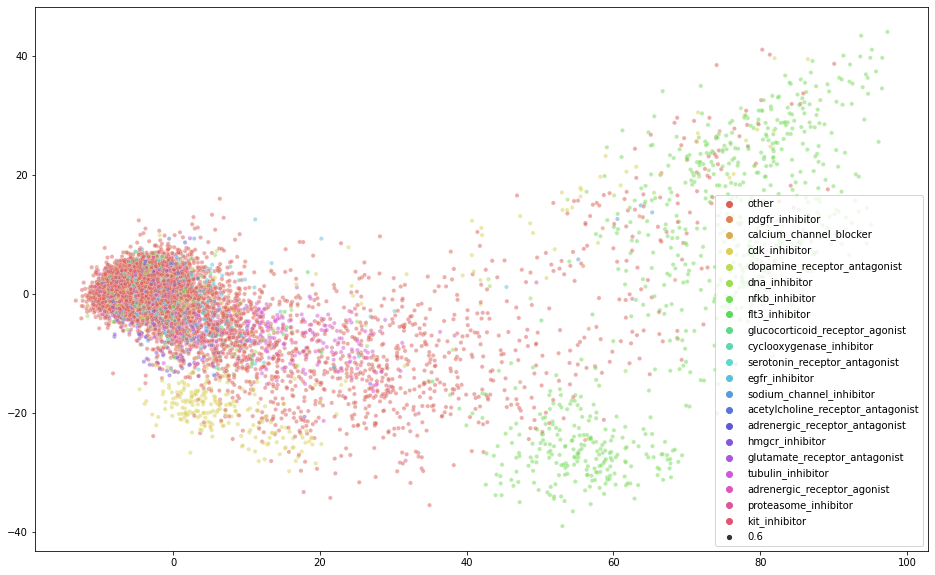
\includegraphics[height=9cm]{images/pca.png}\label{pca map}
% \end{figure}
\subsection{Discussion}
Our analysis demonstrates the existence of a lower biologically relevant linear space achieving some form of separation with respect to the
MoAs. This, however, is not enough to conclude on the actual intrinsic dimensionality of the gene expression and cell viability space. Different cell or tissue types tend to cluster separately and can in principle be connected via a single nonlinear line, hereby complicating the notion of intrinsic dimensionality \cite{lenz_principal_2016}. Additionally, the dimensionality estimation is affected by the selection bias introduced with the dataset as it does not cover the full range of all possible gene expression patterns \cite{lenz_principal_2016}.\\
Biologically, however, we know that genes affect the expression of each other through gene regulatory networks. The number possible network states is hereby limited and therefore significantly lower than the number of genes, implying that the intrinsic dimensionality of the  gene expression space is substantially lower than the number of genes \cite{lenz_principal_2016}.\\ 
When it comes to the MoA inference task that we tackle in the next section, the low cumulative variance captured by the first 100 principal components may suggest that non-linear methods  could achieve better separation of the MoAs.

\chapter{Model Training}\label{model_training}
In this section, we are concerned with learning the functional mapping \(f\) defined in (\ref{funcmap}) and hereby constructing a model that predicts a set of mechanism of actions encoded as a binary vector for a given drug perturbation. 
This task can essentially be described as a \textit{multi-label classification} problem which is a generalization of \textit{multinomial classification} and requires more thought and adaptions in the sampling, learning and evaluation methods than the latter counterpart.\\
\section{Data Partitioning}
In order to obtain an generalizable estimate of the performance of our model, we cannot compute evaluation metrics on the same dataset as was used for training or optimization as this would result in a biased score that is unlikely to generalize to future, unseen data. In the context of drug action prediction, such a biased score would not give us an accurate assessment of the robustness of our model and the ability to predict the MoA for new unknown compounds. 
We therefore partition our dataset \(\mathscr{D}\) into three disjoint subsets: A training set (70\% of the samples) for fitting the parameters of the model, a validation set (15\% of the samples) for optimizing the hyperparameters which are parameters controlling the learning process and finally a test set (15\% of the samples) on which we evaluate the optimized models in order to provide an approximation of the generalization error.\\
% There exists other data partitioning methods such as \textit{cross-validation} in which a dataset is repeatedly split into a training dataset and a validation dataset that have shown to yield higher average predictive performance that simple splitting \cite{schaffer_selecting_1993}. However, it is still debated whether this method also results in less bias. \\
% In our study, the fairly high number of samples reduced the need for cross-validation and our computational restrictions made the expensive cross-validation method rather infeasible. \\
Another requirement for the estimate of generalisation error is that the subsets follow a similar distribution. As shown in Figure \ref{label_dist}, the distribution of labels in our dataset is very imbalanced. This is commonly mitigated using stratified sampling in the partition of the datasets. While the implementation of this method for the multinomial classification problem is clear (e.g. groups are differentiated based on the value of the target variable), it is not evident how this would work for our multi-label case. We employ the novel \textit{iterative stratification} algorithm proposed by Sechidis \textit{et al.}. In each iteration, it greedily examines the label with the fewest remaining examples in order to avoid that samples may be distributed in an undesired way if rare labels are not examined in priority. For each example of this label, it then selects an appropriate subset for distribution according to empirically validated heuristics \cite{sechidis_stratication_nodate}.
\begin{figure}[h!]
\centering
\caption{Distribution of labels}
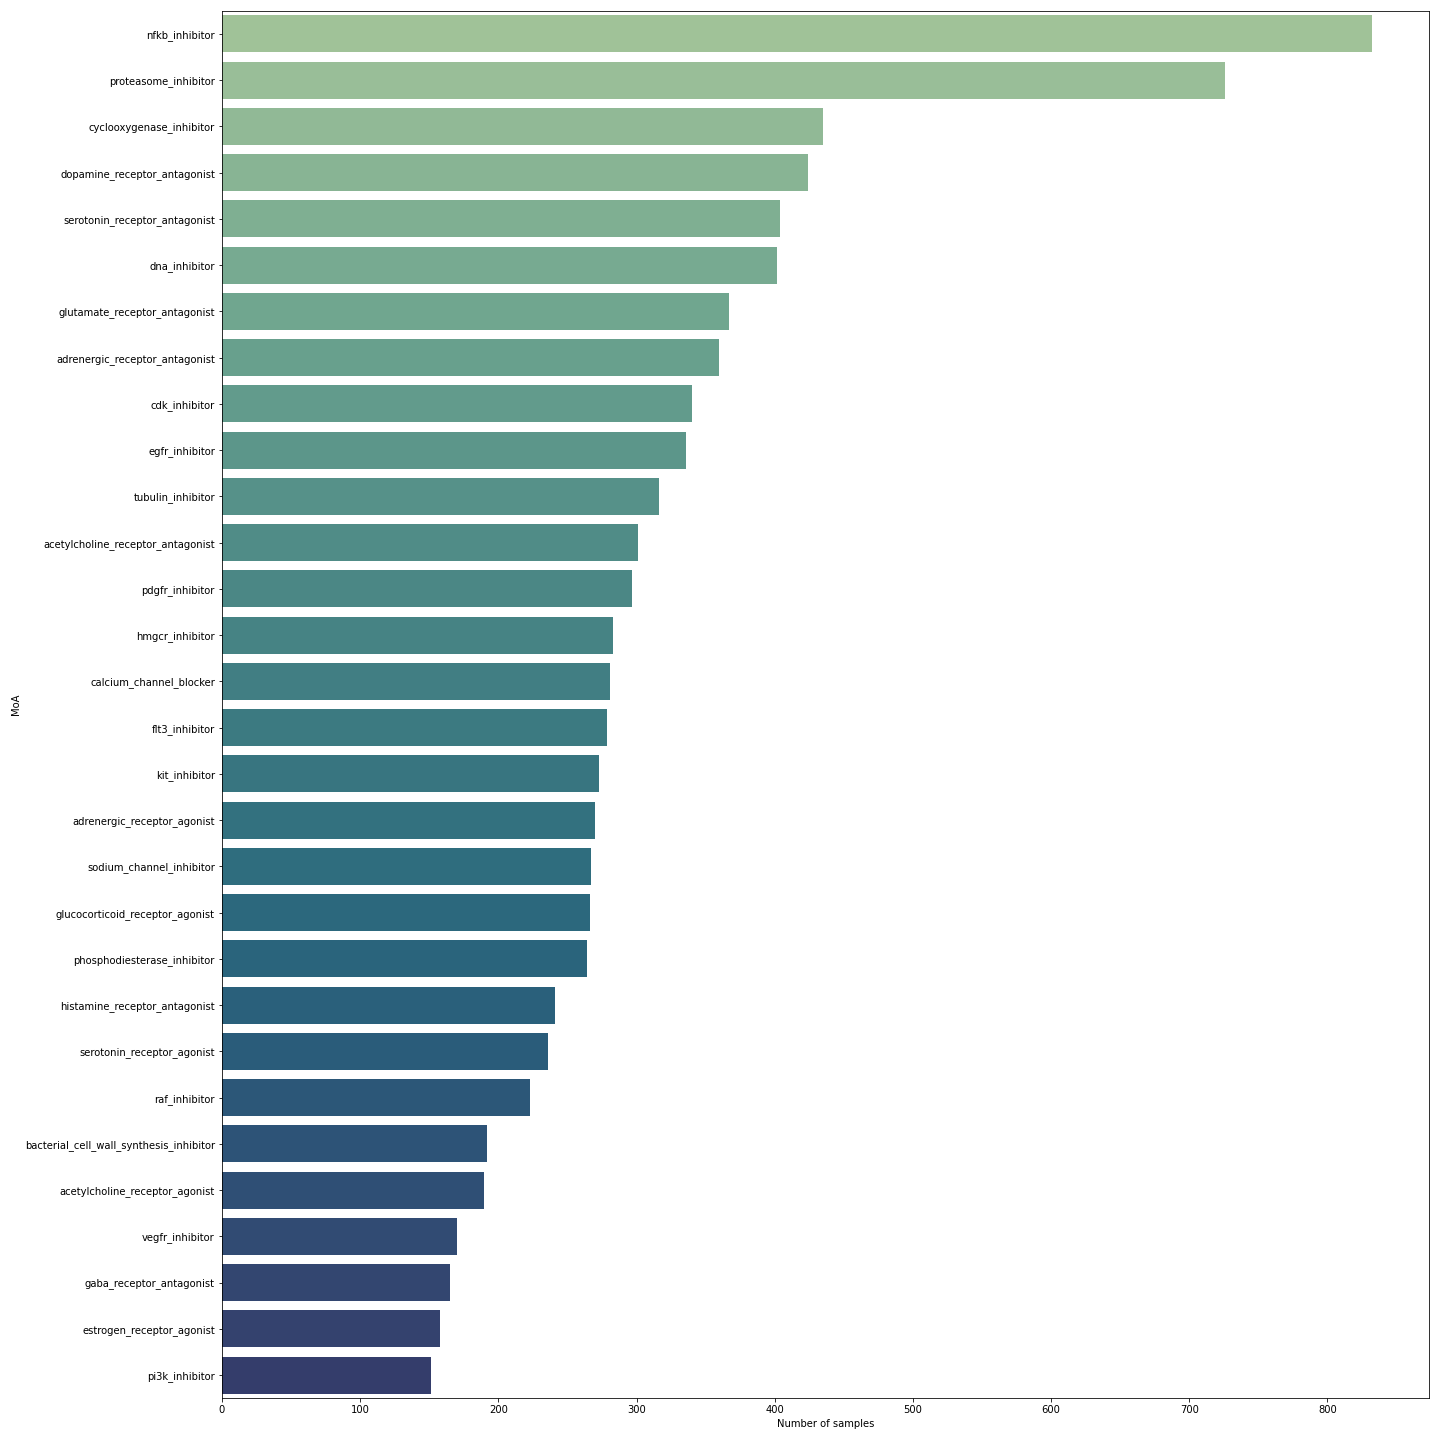
\includegraphics[height=10cm]{images/label_dist.png}\label{label_dist}
\end{figure}
\section{Evaluation Measures}
Evaluation measures are critical to the assessment of the performance of a model and there exists trade-offs between different evaluation measures. Its choice can lead to widely diverging interpretations and is therefore of great importance.

The two desirable outcomes of the classification problem are 
\begin{itemize}
    \item \textit{True Positive}: Correctly predicting that a drug has a certain effect.
    \item \textit{True Negative}: Correctly predicting that a drug does not have a certain effect.
\end{itemize}

The two two types of errors to avoid are:
\begin{itemize}
    \item \textit{False Positive}: Wrongly assigning a specific effect to a drug.
    \item \textit{False Negative}: Failing to predict an effect of a drug.
\end{itemize}

Most metrics used for evaluation of classifiers are a function of these outcomes. In the context of multi-label classification, we additionally need to average the metrics across labels.

Accuracy is the most common evaluation criterion and informally describes the ratio of the number of correct predictions over the total number of predictions:
\[\text { Accuracy }=\frac{T P+T N}{T P+T N+F P+F N}\]

where TP = True Positives, TN = True Negatives, FP = False Positives, and FN = False Negatives.

Accuracy, however, is not well suited to class-imbalanced problems like ours. A classifier can reach high accuracy scores on imbalanced data by merely predicting the majority class. Accuracy does not distinguish between the numbers of correctly classified examples of different classes \cite{galar_review_2012}.

A better indication of model performance is given by the Precision-Recall Curve which demonstrates the tradeoff between precision and recall given by
\[\text { Precision }=\frac{TP}{TP+ FP}\]
\[\text { Recall }=\frac{TP}{TP+ FN}\]
for different thresholds. A high area under the curve (AUC) is desirable as it signifies both high recall and high precision.




\section{Results}
Baselines are critical when approaching a machine learning problem as they guide our further experiments and provide a point of reference from which to compare other algorithms.\\
We implement two different baselines with increasing complexity. The first baseline is a trivial solution and just predicts the most frequent label.
For the second baseline, we chose a simple linear classifier and implemented multinomial regression with a single-layer perceptron with a sigmoidal output activation function.
We trained both baselines on the training set and evaluated the models on the testing set. As seen in Table \ref{baseline_table}, the simple linear classifier strongly outperforms our trivial baseline.

\begin{table}[h!]
\centering
\begin{tabular}{lrrrr}
\toprule
{Model} &  Train Loss &  Test Loss & Train AUC & Test AUC  \\
\midrule
Majority Label Classifier &  0.0801 & 0.0574 & 0.0052 & 0.0037  \\
% Multinomial Regressor  & 0.0128 & 0.0206 & 0.4290 & 0.1075 \\
Multinomial Regressor  & 0.0128 & 0.0131 & 0.429 & 0.402 \\
% 2-Hidden Layer MLP & 0.0080 & 0.017 & 0.6885 & 0.1533 \\
2-Hidden Layer MLP & 0.0080 & 0.011 & 0.6885 & 0.6678 \\
\bottomrule
\end{tabular}
\caption{Results of baselines and improved models}\label{baseline_table}
\end{table}

Given that the ground-truth values of the model are mechanisms of actions which represent rather abstract concepts, we conjecture that additional hidden layers could be helpful for the learning algorithm to learn more abstract and hereby more discriminative representations. 
We therefore construct an extension of the sigmoidal single-layer perceptron by adding two hidden layers with Rectified Linear Units (ReLus). The first hidden layer maps the input features onto a 2048-dimensional latent space and the second hidden layer maps the latter onto a 1048-dimensional latent space. The new MLP achieved an AUC of 0.6678 on the test set. In the next section, we further improve our proposed MLP by jointly optimizing the architecture and hyperparameters  of our model using \textit{Bayesian Optimization}.  

\chapter{Bayesian Hyperparameter Optimization}
Bayesian Optimization (BO) is a popular approach to optimizing objective functions with costly evaluation. It builds a surrogate model for the objective function and quantifies the uncertainty in that surrogate using a stochastic process, in practice usually a Gaussian Process (GP) \cite{frazier_tutorial_2018}.
In the context of our task, the objective function \(f\) is the AUC on the validation set after training our neural network on a set of hyperparameters \(\mathbf{x}\). 
Let \(\mathbf{x}_{1}, \ldots, \mathbf{x}_{n} \in \mathbb{R}^{d}\) be the observed points after \(n\) trials and \(\mathbf{y}_{n}=\left(y_{1}, \ldots, y_{n}\right)^{\top}\) be the corresponding observations of the function \(f\).
By the Gaussian process model, the observation \(y\) for a new set of hyperparameters \(\mathbf{x}\) is normally distributed, \(y \sim \mathcal{N}\left(\mu_n(\mathbf{x}), \sigma_n^{2}(\mathbf{x})\right)\). The predictive mean and  variance functions are defined as:
\[\mu_{n}(\mathbf{x})=\mathbf{k}_{n}(\mathbf{x})^{\top}\left(\mathbf{K}_{n}+\sigma_{n}^{2} \mathbf{I}\right)^{-1} \mathbf{y}_{n}\]
\[\sigma_{n}^{2}(\mathbf{x})=k(\mathbf{x}, \mathbf{x})-\mathbf{k}_{n}(\mathbf{x})^{\top}\left(\mathbf{K}_{n}+\sigma_{n}^{2} \mathbf{I}\right)^{-1} \mathbf{k}_{n}(\mathbf{x}),\]
where
\(\mathbf{k}_{n}(\mathbf{x})=\left(k\left(\mathbf{x}_{1}, \mathbf{x}\right), \ldots, k\left(\mathbf{x}_{n}, \mathbf{x}\right)\right)^{\top}\)
and \(\left(\mathbf{K}_{n}\right)_{i j}=k\left(\mathbf{x}_{i}, \mathbf{x}_{j}\right)\). \(k\) is our chosen kernel function, representing the covariance of a pair of observations. \(k\) is commonly chosen to be an exponentiated quadratic kernel with overall variance \(\sigma^{2}\) and lengthscale \(\ell\) :
\[k\left(\mathbf{x}_{i}, \mathbf{x}_{j}\right)=\sigma^{2} \exp \left(-\frac{\left\|\mathbf{x}_{i}-\mathbf{x}_{j}\right\|^{2}}{2 \ell^{2}}\right)\]

For the purpose of practical hyperparameter optimization, the Matern 5/2 kernel is commonly used as it  allows for less smooth surfaces \cite{snoek_practical_nodate}.
\[k\left(\mathbf{x}_{i}, \mathbf{x}_{j}\right)=\theta_{0}\left(1+\sqrt{5 r^{2}\left(\mathbf{x}_{i}, \mathbf{x}_{j}\right)}+\frac{5}{3} r^{2}\left(\mathbf{x}_{i}, \mathbf{x}_{j}\right)\right) \exp \left(-\sqrt{5 r^{2}\left(\mathbf{x}_{i}, \mathbf{x}_{j}\right)}\right)\]

The Gaussian prior and the observations induce a posterior over functions which help us decide where to next evaluate \(f\) using the inexpensive acquisition function \(a\). The next point \(\mathbf{x}_{n+1}\) is determined via the proxy optimization  \(\mathbf{x}_{n+1}=\operatorname{argmax}_{\mathbf{x}} a(\mathbf{x})\).
A common choice of acquisition function is the \textit{Expected Improvement}
\[
a_{\mathrm{EI}}(x)=\mathbb{E}[f(\mathbf{x})-f_{n}^{*} \mid\left(\mathbf{x}_{1}, y_{1}, \ldots, \mathbf{x}_{n}, y_{n}\right)],
\] where \(f_{n}^{*}\) is the maximal value of \(f\) observed so far.
\section{Experimental Setup}
One of the most crucial aspects of the experimental setup of Bayesian Optimisation is the search space. It involves the choice of the hyperparameters to optimize and their domain and is subject to the trade-off between computational resources and time. Additionally, BO currently has scalability issues and is practically limited to a search space involving 10 - 20 parameters \cite{moriconi_high-dimensional_2020}.

We take a heuristic approach to the optimization of the neural network architecture by defining three parameters that describe the entire architecture rather than exploding the dimensionality of the search space with parameters describing the activation functions and number of nodes for each layer of the network:
\begin{itemize}
    \item The activation function for all hidden layers.
    \item The number of hidden layers in the network.
    \item The \textit{node decreasing factor} describing the decrease in the number of nodes from layer to layer. Let \(|l_i|\) be the number of nodes in layer \(i\), where \(l_0\) is the input layer, and \(d\) be the node decreasing factor, then the number of nodes layer \(i\) are described by \( |l_i| = d|l_{i-1}| \).
\end{itemize}
This relaxed neural architecture optimization follows from the assumption that the number of nodes need to decrease in order to learn biologically meaningful and discriminative generalisations of the correlated biological data. \\
Aside from architecture parameters, we optimize the 
\begin{itemize}
    \item batch size indicating how many samples are used for each parameter update.
    \item epochs (i.e. the number of full training cycles on the data set).
    \item learning rate of the gradient optimization.
    \item the dropout rate for regularization.
    \item boolean parameter indicating whether \textit{batch normalization} should be applied to the layers. Batch normalization standardizes the activations of each input variable per mini-batch with the aim of stabilizing and speeding-up the learning training procedure.\\
\end{itemize}

Table \ref{search_sapce} shows the search space including the domain of each parameter.

\begin{table}[h!]
\centering
\begin{tabular}{lrrrr}
\toprule
{Hyperparameter} &  Domain  \\
\midrule
Hidden layers & {1,2,3} \\
Node decreasing factor & [0.2,0.95] \\
Activation function & {ReLU, SeLU, Swish} \\
Batch size & {32,64,128,256} \\
Epochs & {15,35,45} \\
Dropout & [0.1,0.8] \\
Learning rate & [1e-6,1e-1]  \\
Batch normalization & {True, False} \\
\bottomrule
\end{tabular}
\caption{Domain for hyperparameter optimization}\label{search_sapce}
\end{table}

\section{Results}
We performed 74 training runs with parameters sampled according to the acquisition function and evaluated the runs on the validation set. The best parameters according to the validation performance are shown in Table \ref{bo_results}.
The set of parameters achieved a validation AUC of 0.7342 and a test AUC of 0.7215.
\begin{table}[h!]
\centering
\begin{tabular}{lrrrr}
\toprule
{Hyperparameter} &  Best value  \\
\midrule
Hidden layers & 2 \\
Node decreasing factor & 0.78 \\
Activation function & ReLU \\
Batch size & 32 \\
Epochs & 35 \\
Dropout & 0.22 \\
Learning rate & 0.0017  \\
Batch normalization & False \\
\bottomrule
\end{tabular}
\caption{Best parameters identified by BO}\label{bo_results}
\end{table}
% \begin{figure}[h!]
% \centering
% \caption{Evaluations of BO}
% 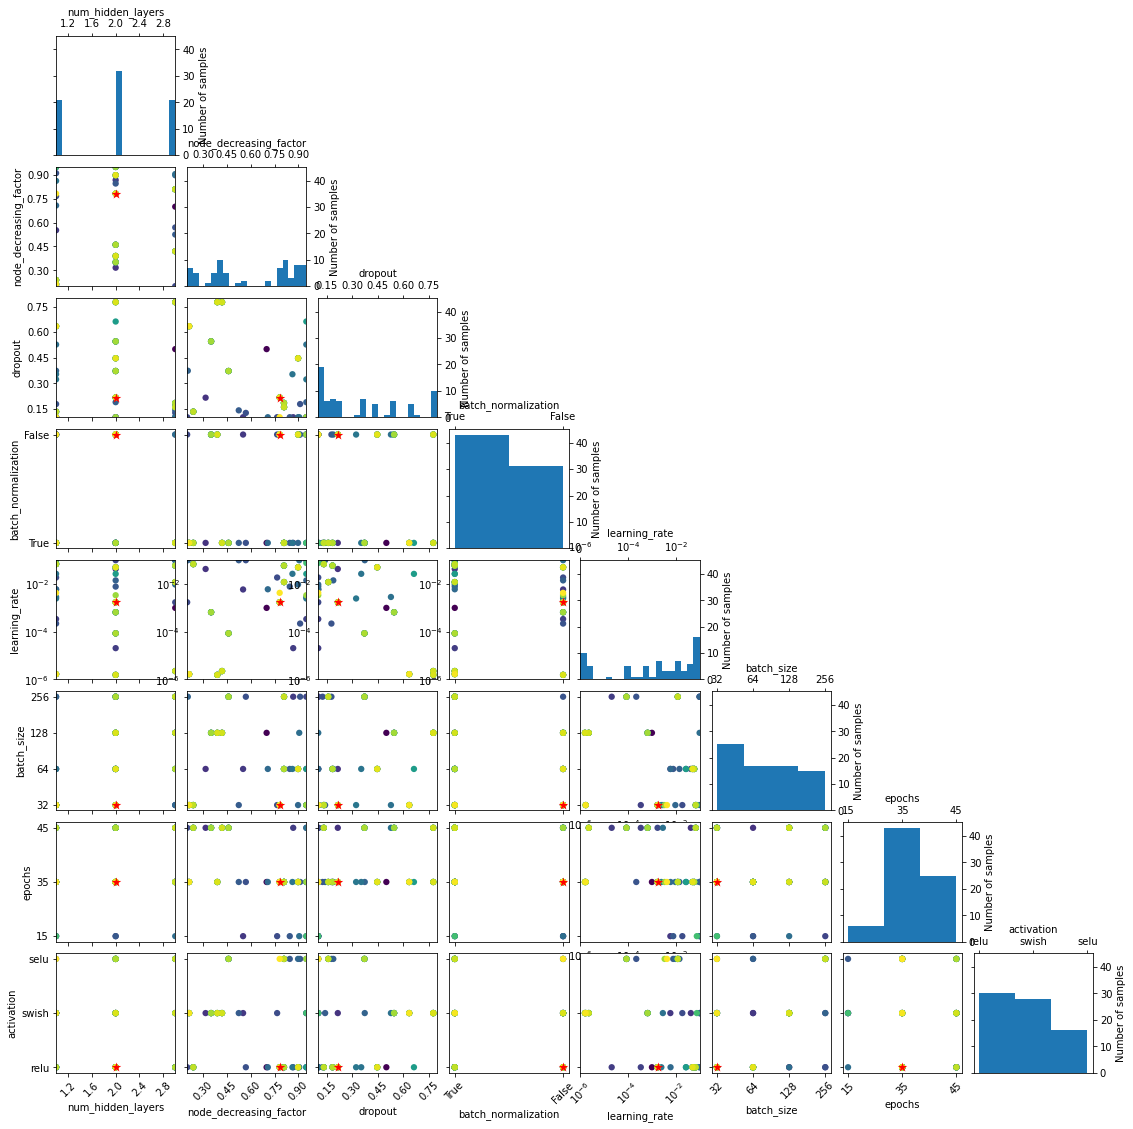
\includegraphics[height=16cm]{images/bo_evaluations.png}\label{bo_eval}
% \end{figure}
Figure \ref{bo_obj} shows the partial dependence plot of the objective function and is calculated by averaging the value of the objective function a set of random samples in the search-space, while keeping one or two dimensions fixed at regular intervals. 
\begin{figure}[h!]
\centering
\caption{\textbf{Partial dependence plots of objective function.} Yellow regions are better and blue regions are worse, the red star indicates the optimum of the objective function.}
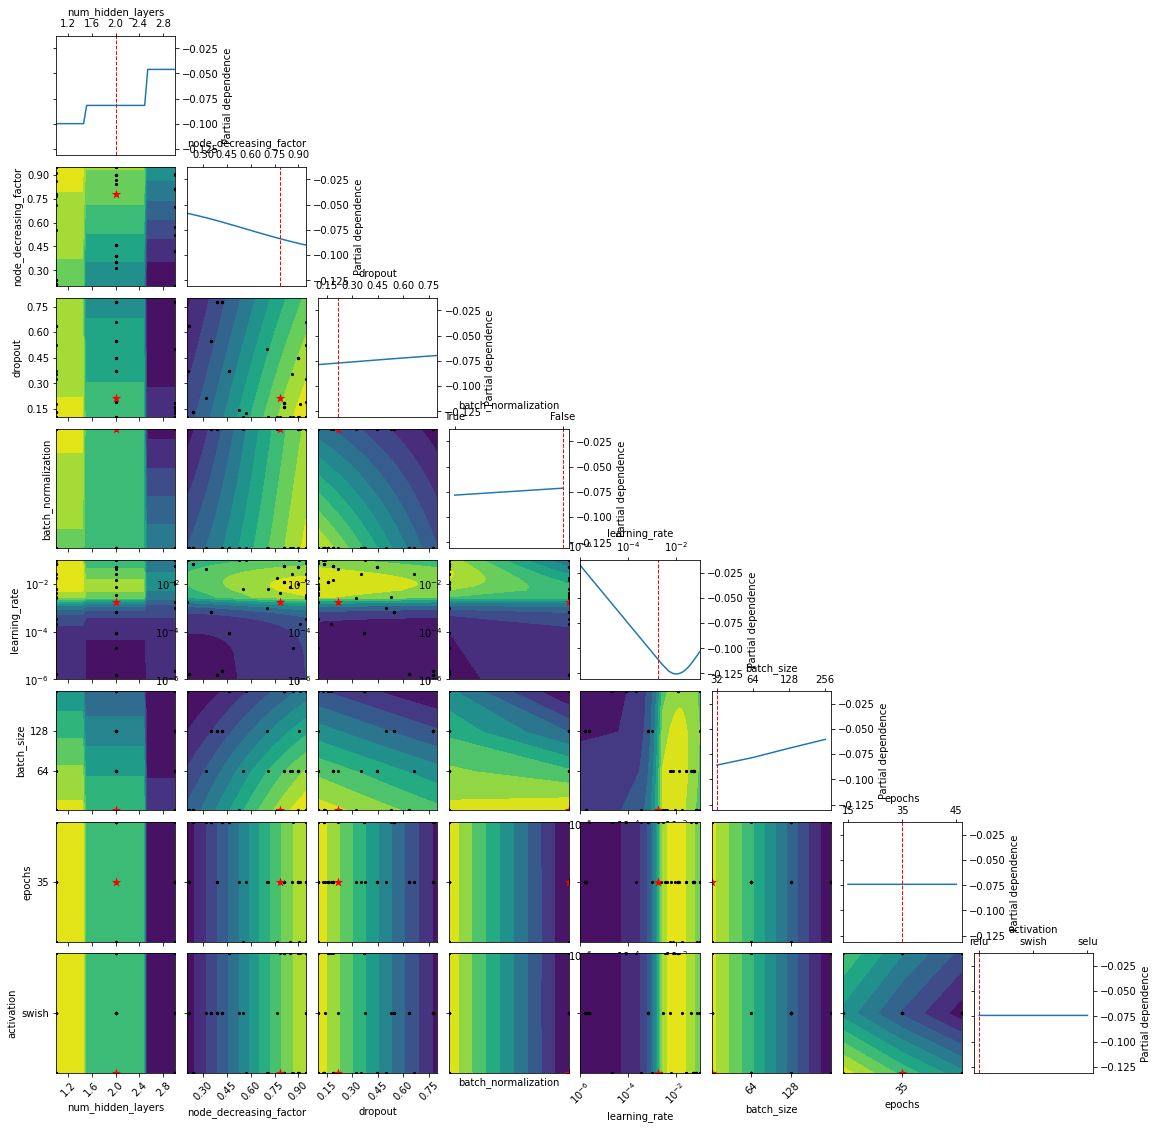
\includegraphics[height=16cm]{images/bo_objective.png}\label{bo_obj}
\end{figure}
\section{Discussion}
The dependence plots indicate that a smaller number of hidden layers with a high node decreasing factor are favoured, while the node decreasing factor becomes increasingly important with the number of hidden layers.\\
We performed relaxed neural architecture search using a constant node decreasing factor, hereby assuming the optimal number of nodes to be exponentially decaying in the number of layers. In further experiments, we could extend the node decreasing factor to be a different function of the number of layers.\\
In addition to these observations, we note that a smaller number of hidden layers is favoured, irrespective of the activation function, epochs or dropout rate but respective of the learning rate. Only smaller learning rates (\(10^{-2}\)) seem to differentiate the performances for hidden layer sizes. This could be due to the fact that larger hidden layer sizes induce a more complex error surface that is more difficult to navigate in a meaningful way in the gradient optimization when faced with a too large learning rate. \\

Finally, it should be noted the surrogate model and dependence plots can be inaccurate because they are built from only 74 samples of calls to the fitness function. The results should be validated on a larger set of trials.


\chapter{Model Interpretation}
One of the biggest obstacles to the adoption of deep learning in biomedical applications is its lack of interpretability. Without the interpretabiliy criterion met, physicians and other medical professionals cannot justify taking a decision based solely on the output of a black box algorithm as patients' lives may be at stake. In the context of our work, understanding why a compound is attributed a certain mechanism of action and which genes, pathways and biological processes led to the classification is critical to being able to move forward with the costly and sensitive drug development process. Interpretability further ensures that a neural network bases its predictions on reliable representations and signals of the data. Finally, we are interested in the patterns identified by the neural network and whether they are able to generate new biological insights.

\section{Integrated Gradients}
In this section, we want to investigate why a specific compound was assigned a particular mechanism of action and how it achieves that particular MoA.
For instance, the MoA of anti-inflammatory drugs such as Aspirin and Ibuprofen is \textit{cyclooxygenase inhibitor} which describes the inhibition of the inflammation inducing cyclooxygenase enzymes. However, the way Ibuprofen and Aspirin achieve the inhibition of these enzymes can involve completely different pathways and biological processes. Identifying these can help us assess the efficacy, safety and side effects of the drug.

Recent works in methods for interpreting deep neural networks show that gradient methods produce better interpretations of a neural network than simple weight analysis \cite{montavon_methods_2018}. Backpropagating the activation of the output neuron and analysing the product of the gradient and feature values is a reasonable start for feature attribution \cite{baehrens_how_nodate}.\\
However, gradients can be problematic when activations have a near-zero gradient at high or low inputs such as with the ReLU activation function \cite{shrikumar_not_2017}. The prediction function may flatten at the input and thus have zero gradient despite the significance of the input.
\textit{Sundararajan et al.} \cite{sundararajan_axiomatic_2017} formalize this requirement to feature attribution methods as the \textit{Sensitivity Axiom}. They establish that "an attribution method satisfies Sensitivity if for every input and baseline that differ in one feature but have different predictions, then the differing feature should be given a nonzero attribution" \cite{sundararajan_axiomatic_2017}.
Several methods were proposed to tackle this issue. The \textit{DeepLift} method, for instance, satisfies the sensitivity axiom by computing feature importance based on the difference in activation from a baseline or reference input which may still be nonzero even when the gradient is zero \cite{sundararajan_axiomatic_2017}.\\
Unfortunately, these improved methods violate another requirement of attribution methods, namely \textit{Implementation Invariance}. The axiom of Implementation Invariance states that attributions for two functionally equivalent networks, i.e., structurally different networks producing the same outputs for every input, should be equivalent. Its violation implies that attributions of these methods are potentially sensitive to unimportant aspects of the model. \cite{sundararajan_axiomatic_2017}. \\
Integrated Gradients, a method proposed by \textit{Sundararajan et al.}, addresses these issues by defining an attribution value for each feature by considering the integral of the gradients taken along a straight path from a baseline instance \(x^{\prime}\) to the input instance \(x\) \cite{sundararajan_axiomatic_2017}. \\

We define this formally for our problem of identifying the integrated gradients of the gene and cell values for a given MoA classification.

For our learned function, \[f: \mathbb{R}^{L} \rightarrow \mathbb{R}^{K},\] we define \[f_{k}: \mathbb{R}^{L} \rightarrow \mathbb{R}\] as a mapping to the probability of the indexed label \(k\), which could be one of the ground-truth MoA labels. The attributions \(A_{k}^{(i)}\left(\mathbf{x}, \mathbf{x}^{\prime}\right)\) towards the label \(k\) for each feature \(x_{i}\) with respect to the corresponding feature \(x_{i}^{\prime}\) in the baseline are calculated as
\[ A_{k}^{(i)}\left(\mathbf{x}, \mathbf{x}^{\prime}\right)=\left(x_{i}-x_{i}^{\prime}\right) \int_{0}^{1} \frac{\partial f_{k}\left(\mathbf{x}^{\prime}+\alpha\left(\mathbf{x}-\mathbf{x}^{\prime}\right)\right)}{\partial x_{i}} d \alpha \]

\section{Results}
For our experimental setup, we select samples for different labels uniformly at random and compute the attributions for each gene and cell feature with respect to the mean control perturbation as baseline.

In order to select the features with highest attributions towards the MoA label for further analysis, we cannot just take the absolute values of the attributions as this would lead to misleading results. For instance, a negative attribution could both signify the down-regulation of a gene contributing to the label attribution and the up-regulation of a gene negatively contributing to the label attribution. It is imperative to keep the former and remove the latter from our selection.

We filter our array of attributions by only keeping the attributions where the sign of the integrated gradient matches the sign of the feature activation.

We then select a subset of the 50 highest absolute attributions and extract the gene identifiers to perform \textit{Reactome} pathway enrichment analysis \cite{fabregat_reactome_2017}. Reactome is a peer-reviewed pathway database and the enrichment provides us with the statistically over-represented pathways in which the genes in the subset are involved, hereby enabling a biological interpretation of the integrated gradients.
We then compare the statistically significant (\(p < 0.05\)) pathways with literature associating these pathways with the drugs used in the respective samples.

In order to quantify our results, we define an enrichment of the attributions of a drug sample as being confirmed by the literature if in the 5 pathways with highest statistical significance,  at least 2 pathways are found to be associated with the drug and its MoA in the literature.

We conduct the above described method on a set of 20 samples with distinct MoA. The MoAs with highest label count were selected in order to mitigate overfitting caused by MoA with very few samples in the training set. We report a confirmation of enrichment for 9 out of 20 samples. 


We demonstrate our method on an example perturbation sample by \textit{Bortezomib} and its associated target \textit{Proteasome Inhibitor.} Proteasomes are protein complexes which degrade unneeded or damaged proteins by proteolysis. The proteasome pathways are critical for the proliferation and survival of all cells and appear to be associated with the pathophysiology of some cancers. It was therefore suggested that pharmacological inhibition of proteasome function may prove useful as a novel class of anticancer drugs \cite{chen_bortezomib_2011}. The proteasome inhibitor Bortezomib has shown to induce apoptosis of a variety of cancer cells, including leukemia, lymphoma, multiple myeloma and breast cancers \cite{cao_ubiquitin-proteasomal_2011}.
Table \ref{bortezomib} shows the 5 most significant pathways for the gene attributions. We compared the identified pathways with the literature on the pharmacodynamics of Bortezomib and could find at least two pathway associations in the literature. 
The over-represented Telomere pathways in Table \ref{bortezomib} align with findings by \textit{Weiss et al.} that Bortezomib downregulates telomerase activity in multiple myeloma cells \cite{weiss_differential_2012}.
We further find confirmation in the literature for the importance of \textit{Histone deacetylases} (HDACs) as found by our over-representation analysis. Histone deacetylases are enzymes involved in chromatin compaction and transcriptional repression \cite{yang_rpd3hda1_2008}. \textit{Kikuchi et al.} conclude that Histone deacetylases are critical targets of bortezomib-induced cytotoxicity in multiple myeloma \cite{kikuchi_histone_2010}.\\
\begin{table}[h!]
\centering
\begin{tabular}{p{8cm}p{1.5cm}p{1.5cm}p{1.5cm}p{1.5cm}}
\toprule
Pathway name &	\#Entities found &	\#Entities total &	Entities ratio &	Entities p-Value\\
\midrule
Telomere Maintenance&	3&	111&	0.0075	&0.0009 \\
Chromosome Maintenance&	3&	138 &	0.0094&	0.0018 \\
TGFBR2 MSI Frameshift Mutants in Cancer &	1 &	2&	0.0001&	0.0035 \\
E3 ubiquitin ligases ubiquitinate target proteins&	2&	61&	0.0041&	0.0052\\
HDACs deacetylate histones&	2&	67&	0.0045&	0.0062\\
Extension of Telomeres&	2&	69&	0.0046&	0.0066 \\
\bottomrule
\end{tabular}
\caption{\textbf{Enriched pathways for Bortezomib.}  The columns indicate how many entities (e.g. genes, proteins) are part of the pathway in total and how many where matched. The p-value provides an indication on the probability that the entities matched by chance only.}\label{bortezomib}
\end{table}
\section{Discussion}
The feature attribution method yields relevant biological  interpretations and contributes towards the goal of interpretability in pharmacological prediction models. However, we should note that the results reported above should be validated by further experiments. We conducted our method on a set of only 20 samples as our work is severely time-limited and the method requires significant manual evaluation for the literature research.
Furthermore, it should be noted that the 45\% confirmation ratio for our samples does not suggest that the model or the integrated gradients method is unreliable  as our model looks for correlations between the output and the input and not for causal relationships. Enriched pathways that are not confirmed by the literature could either be indirectly correlated with the MoA or exhibit an unknown causal relationship.  Many drugs are still objects of active research and it is very possible that relationships proposed by our model will be confirmed by research community in the future. \\
Additionally, we should also consider that biological databases such as Reactome are by no means perfect representations of biological knowledge. A lot of information will be missing and hence not appear in our enrichment analysis. \\
Lastly, both positive and negative results are implicated by overfitting and training bias as demonstrated in \ref{model_training}. Especially mechanisms of actions with a lower number of samples in the training set could produce pathway enrichments that are related to noise in the sample and not a significant biological function. \\
We therefore conclude that the proposed model interpretation method should not be used as a tool to evaluate the reliability and robustness of the model but rather as a tool for biological discovery that can generate biological hypotheses  and propose new drug effects that are then to be investigated and experimentally confirmed by biologists.




% We tackle this problem by determining the genes and cells that most contributed to the classification in the the neural network and then enrich these features with annotations from biological process and pathway databases. 


% By identifying the genes and cells that most contributed to the MoA classification, we can infer which biological processes achieve that MoA and whether we can i

% This question is of interest because it  I.e. we want to identify the biological processes


\chapter{Conclusion}
This thesis presented deep learning strategies to identify novel drug targets. The study leveraged the recent availability of transcriptomic drug perturbation data to develop methods of inferring the mechanism of action of compounds, as to identify novel targets for both existing drugs and unknown compounds.\\
In chapter 4, it was shown in the correlation and principal component analysis that linear representations yield biologically relevant interpretations with respect to the activity and function of drug compounds.\\  However, we showed in chapter 5 and 6 that non-linear methods, especially deep neural networks, achieve considerable performance in the MoA prediction task. We further demonstrated how Bayesian optimization can be used in NNs to optimize learning parameters and the architecture. \\
The \textit{Integrated Gradients} method presented in chapter 7 proved to be a promising tool to generate biological hypotheses about drugs and their effects to be investigated by biologists.\\
From a practical perspective, the experiments and results in this project provided a good starting point in leveraging transcriptomic data to identify novel drug targets. However, this problem would benefit from a holistic approach that incorporates inductive biases acquired in biomedical and pharmaceutical research, as well as further data on the chemistry of compounds and physiology of diseases. 
% Include domain specific data

% Limitations
% CMap comes with some limitations, such as limited drug perturbation data, a limited drug coverage, dosage-dependent conditions and the uncertainty of applying cell lines or animal model expression patterns to human systems. Also, the methodology can be expensive and time-consuming before it can generate a significant portion of all safe dosage conditions for a limited number of cell lines for CMap

% use the following and \cite{} as above if you use BibTeX
% otherwise generate bibtem entries
\bibliographystyle{plain}
\bibliography{references.bib}

\end{document}
